% cs296_report_21.tex - A Document about the newly inserted box2d elements
\documentclass[11pt]{article}

\usepackage[top=1in,bottom=1in,left=0.5in,right=0.5in]{geometry}
\usepackage{graphicx}
\usepackage{amsmath}
%\usepackage{mathptmx}

\begin{document}
 % top matter
\title{Project Report: Pinball Simulation}
\author{1.Adit Kabra\\
          120050034\\
          \texttt{kabraadit@cse.iitb.ac.in}\\
        2.Aditya Nambiar\\
          12D070012\\
          \texttt{adityan@cse.iitb.ac.in}\\
        3.Rajesh Roshan Behera\\
          120050079\\
          \texttt{rajeshrb@cse.iitb.ac.in}\\}
\date{\today}
\maketitle
\newpage
\tableofcontents

\newpage
\section{Introduction}
In this project we have created a simulation of a Pinball Game. We have created and designed it in C++ using Box2D library.
We have profiled the code using perf . In this report we have given a gist of our design, its salient features and working. Also this report
gives the observations on the profiling of the code and the possible optimizations that can be done.


\section{Design Of The Simulation}
This section explains the original design planned in for the simulation, the final
design prepared and the changes done. It reflects on the salient features of Box2D library we have utilized in our simulation and various important elements, which are a part of the simulation. The original design that was created, was not a very specific design and was a mere reproduction of the original pinball. Thus the design was created without much knowledge of Box2D. The actual design although does accomplish most of the features of the original pinball within the limitation of Box2D
\subsection{Original Planned Design Of Simulation}
\begin{center}
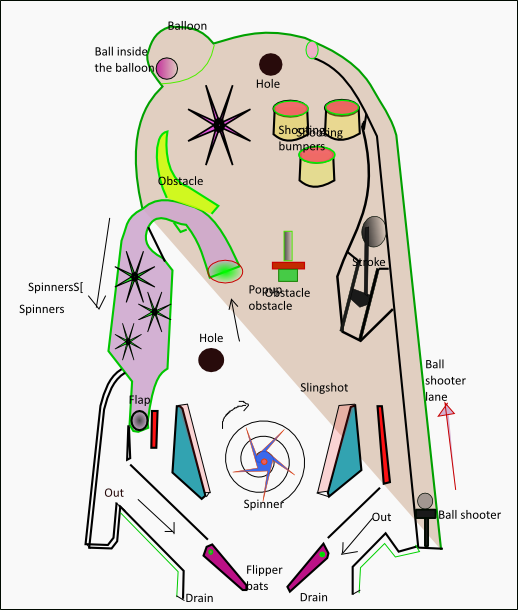
\includegraphics[scale=0.5]{../plots/our.png}\\
Original Design
\end{center}
This image was created using InkScape.\\



\subsection{Actual Design}
\begin{center}
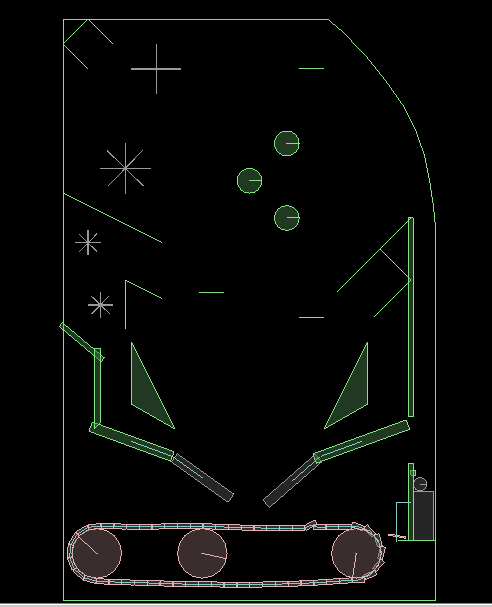
\includegraphics[scale=0.5]{../plots/full.png}\\
Actual Design
\end{center}
In this simulation we launch the ball using the launcher located at the bottom right corner by pressing the button l. Once the ball is inside the main game
it may hit any of the obstacles and behave according to laws of physics. The coefficient of restituion of the triangles and the shrinking balls have been given reasonably high vales to increase the speed of the game. When the flippers miss the ball, the ball falls on the horizontal bar below the flippers and the ball is automatically is brought back to the launcher. Along with the simulation the score is displayed on the top left corner.\\

\subsection{Difference between Original and Actual Design}
1. Hole\\
Hole has been implemented in a different manner. There are like two pipes, the ball goes through one and comes out through other with high speed. \\
2. Removed the obstacle\\
We have eliminated the stroke since we felt that it did not add much value to the simulation. \\
3. Conveyer Belt\\
Implemented the conveyer belt that automatically takes the ball to the launcher for the start of a new game. This was not mentioned in the design, but we got this idea later and hence used it. The gears for conveyer belt are given some angular impulse at the beginning of the game. The boxes are connected using revolute joint to form the chain. The ball, when hits the chain, is given some horizontal velocity to take it to the launcher.\\
4. Spinner Repositioning \\
We removed the spinner between the two triangle bumpers since we felt it looked clumsy. Instead we have placed two spinners at the top of the pinball box.\\
5. Breaking Objects\\
We have inserted three edgeshaped bodies, which break when ball hits them, and the player scores points in doing so. These bodies after breaking fall down, and while falling down do not interact with any body.

\section{Key Elements and obstacles}
\subsection{Flippers}
\begin{center}

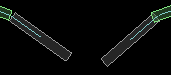
\includegraphics[scale=0.5]{../plots/flippers.png}\\
Flippers
\end{center}
These are the main elements of the the game , which allows the users to direct the ball where ever they want and also to prevent the ball from slipping to the bottom of the game. Pressing 'a' activates the left flipper and key 'd' activates the right flipper.

\subsection{Triangles}
\begin{center}
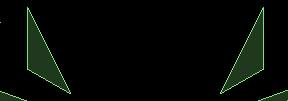
\includegraphics[scale=0.5]{../plots/triangles.jpg}\\
Triangles
\end{center}
These are basically used to throw the ball up since they have high coefficient of restitution and hence the ball bounces off rapidly after colliding with them. 

\subsection{Breaking Object}
There are three edge shaped static bodies, which break down when ball hits them. The player scores points by hitting these objects. After breaking they fall down in simulation, and while falling down do not interact with any other body in the simulation.

\subsection{Dark-Hole}
\begin{center}
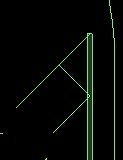
\includegraphics[scale=0.5]{../plots/darkhole1.png}\\
Darkhole where ball goes inside
\end{center}
\begin{center}
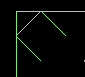
\includegraphics[scale=0.5]{../plots/darkhole2.png}\\
Darkhole from where ball comes out
\end{center}
This is one of the magical features of this pinball simulation. When the ball enters it it comes out the top left corner with great speed. Hence they allow the ball to travel all over the board. They have been implemented by killing the ball when it comes in contact with the dark hole and regenerating it in the top left corner.

\subsection{Spinner}
\begin{center}
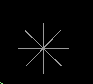
\includegraphics[scale=0.5]{../plots/spinner.png}\\
Spinner
\end{center}
These spinners rotate rapidly when the ball collides with them . They reduce the speed of the ball on collision however are beautiful to watch.

\subsection{Launcher}
\begin{center}
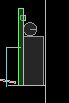
\includegraphics[scale=0.5]{../plots/launcher.png}\\
Launcher
\end{center}
It used to launch the ball with high speed into the simulation. It can be activated by pressing the 'l' key.

\subsection{Conveyer Belt}
\begin{center}
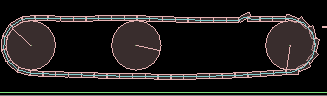
\includegraphics[scale=0.5]{../plots/conveyer.png}\\
Conveyer
\end{center}
Makes the game more automated. Once the player loses the game, after he misses hitting the ball via flippers, it hits the conveyer belt which is just below the flippers. The ball loses its vertical velocity after hitting the flippers, and gains velocity in horizontal direction to move towards the launcher. The conveyer belt throws the ball to Vertical Ball Lifter.

\subsection{Vertical Ball Lifter}
When the ball slips out the flippers it falls on the conveyer belt below the flippers. Then the ball automatically slides and falls on the vertical ball lifter. The vertical ball lifter lifts the ball and places it on the launcher enabling the user to play the game once more! The automization has been achieved using contactlistners .


\subsection{Bumpers}
\begin{center}
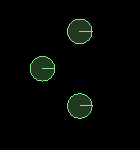
\includegraphics[scale=0.5]{../plots/bumperballs.png}\\
Bumper Balls
\end{center}
Bumpers are nothing but three circular shaped bumpers . When the ball collides with the bumpers they shrink and expand and push the ball away . The ball after the collision achieves a very high speed. The shrinking effect has been achieved by killing the object and regenerating it using contactlisteners to detect if the collision involved Bumpers.

\subsection{Ball}
The main element of the pinball simulation. It can be launched into the games with the help of the launcher by pressing the key 'l'.

\section{Profiling Report}
As our project is a game, there is a lot of keyboard control in the simulation. Due to this reason, the profiling was done including gui. Hence the maximum call, according to the profiling report is done in functions of gui.
\begin{center}
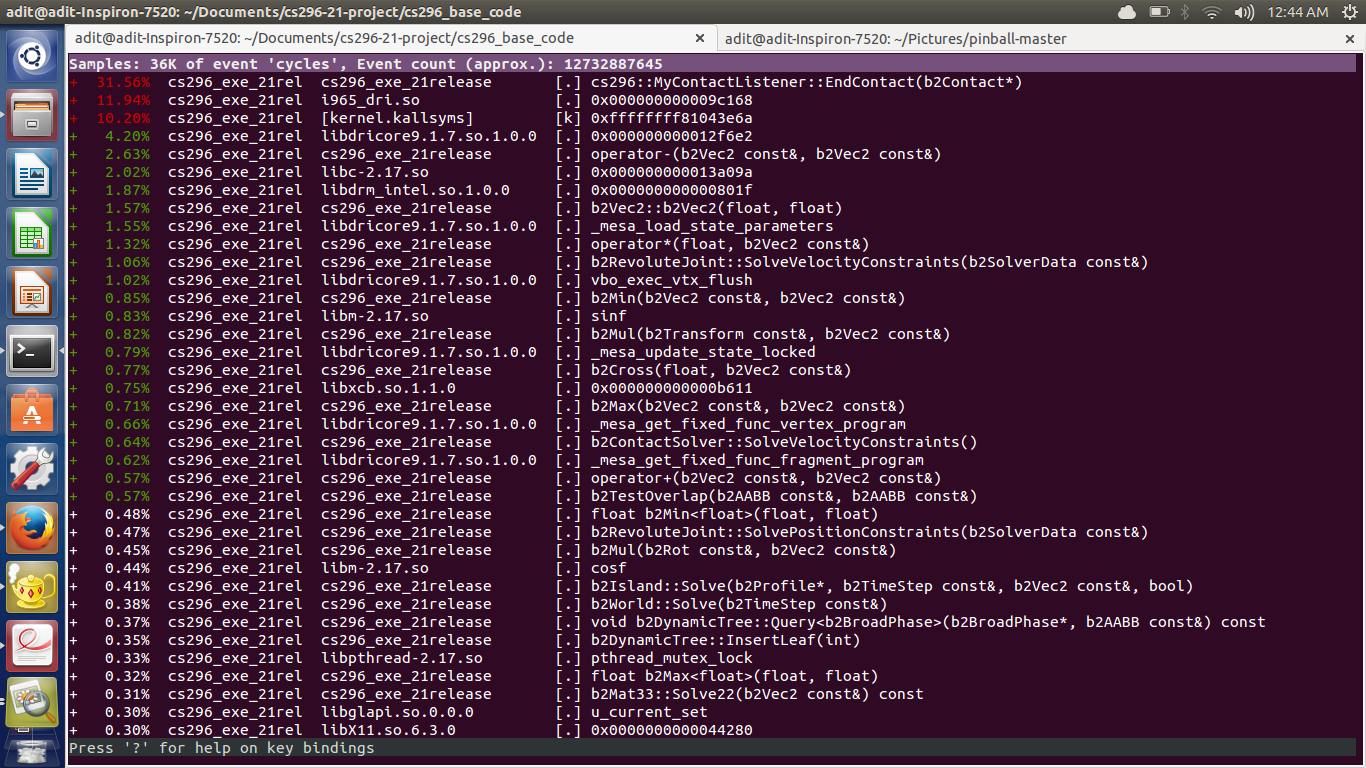
\includegraphics[scale=0.5]{../plots/release.png}\\
Release Profiling Report
\end{center}
\begin{center}
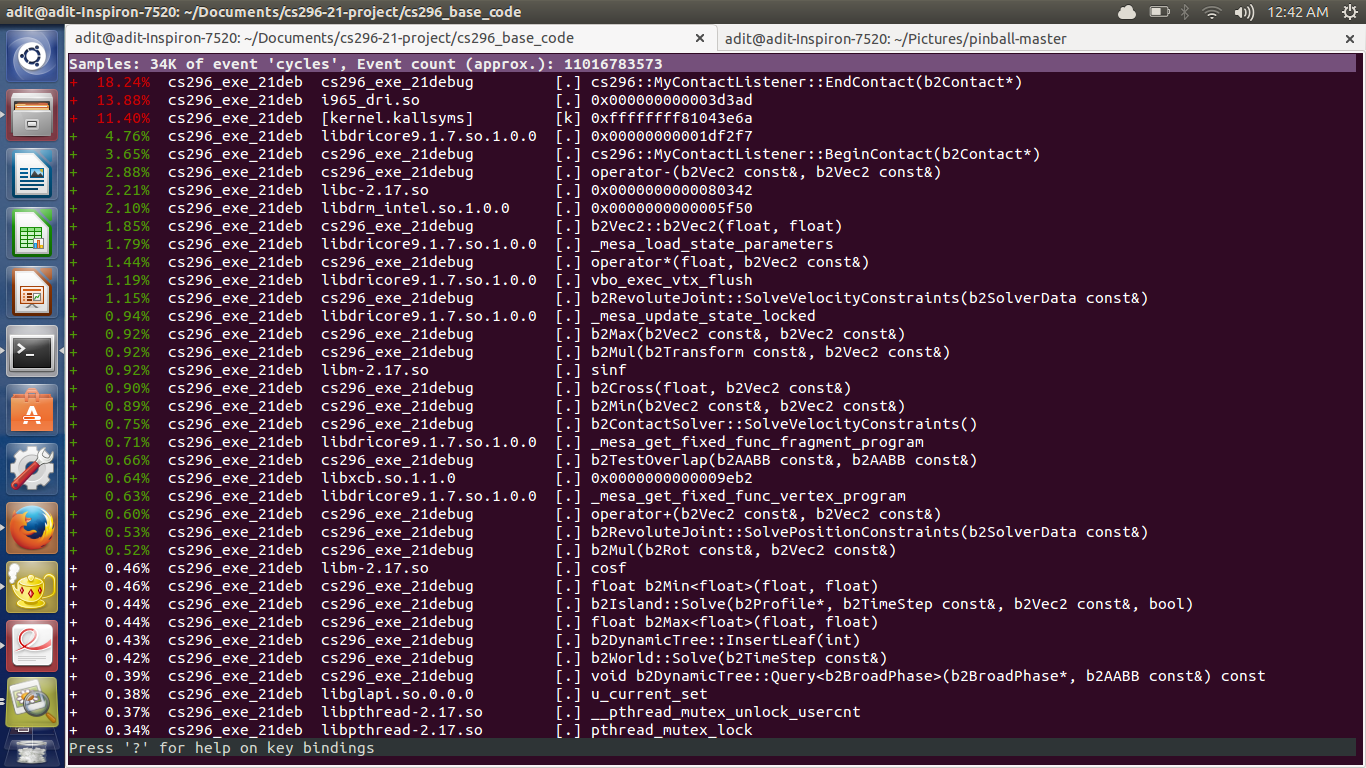
\includegraphics[scale=0.5]{../plots/debug.png}\\
Debug Profiling Report
\end{center}
Besides, both Debug and Profile analysis is quite similar. Both have most percentage of calls to contactlistener, as we have used a lot of times the contact listener function, whenever the ball strikes an object in the game. Hence, these two are the most occuring functions in profiling. And there is not much optimization possible.
\begin{center}
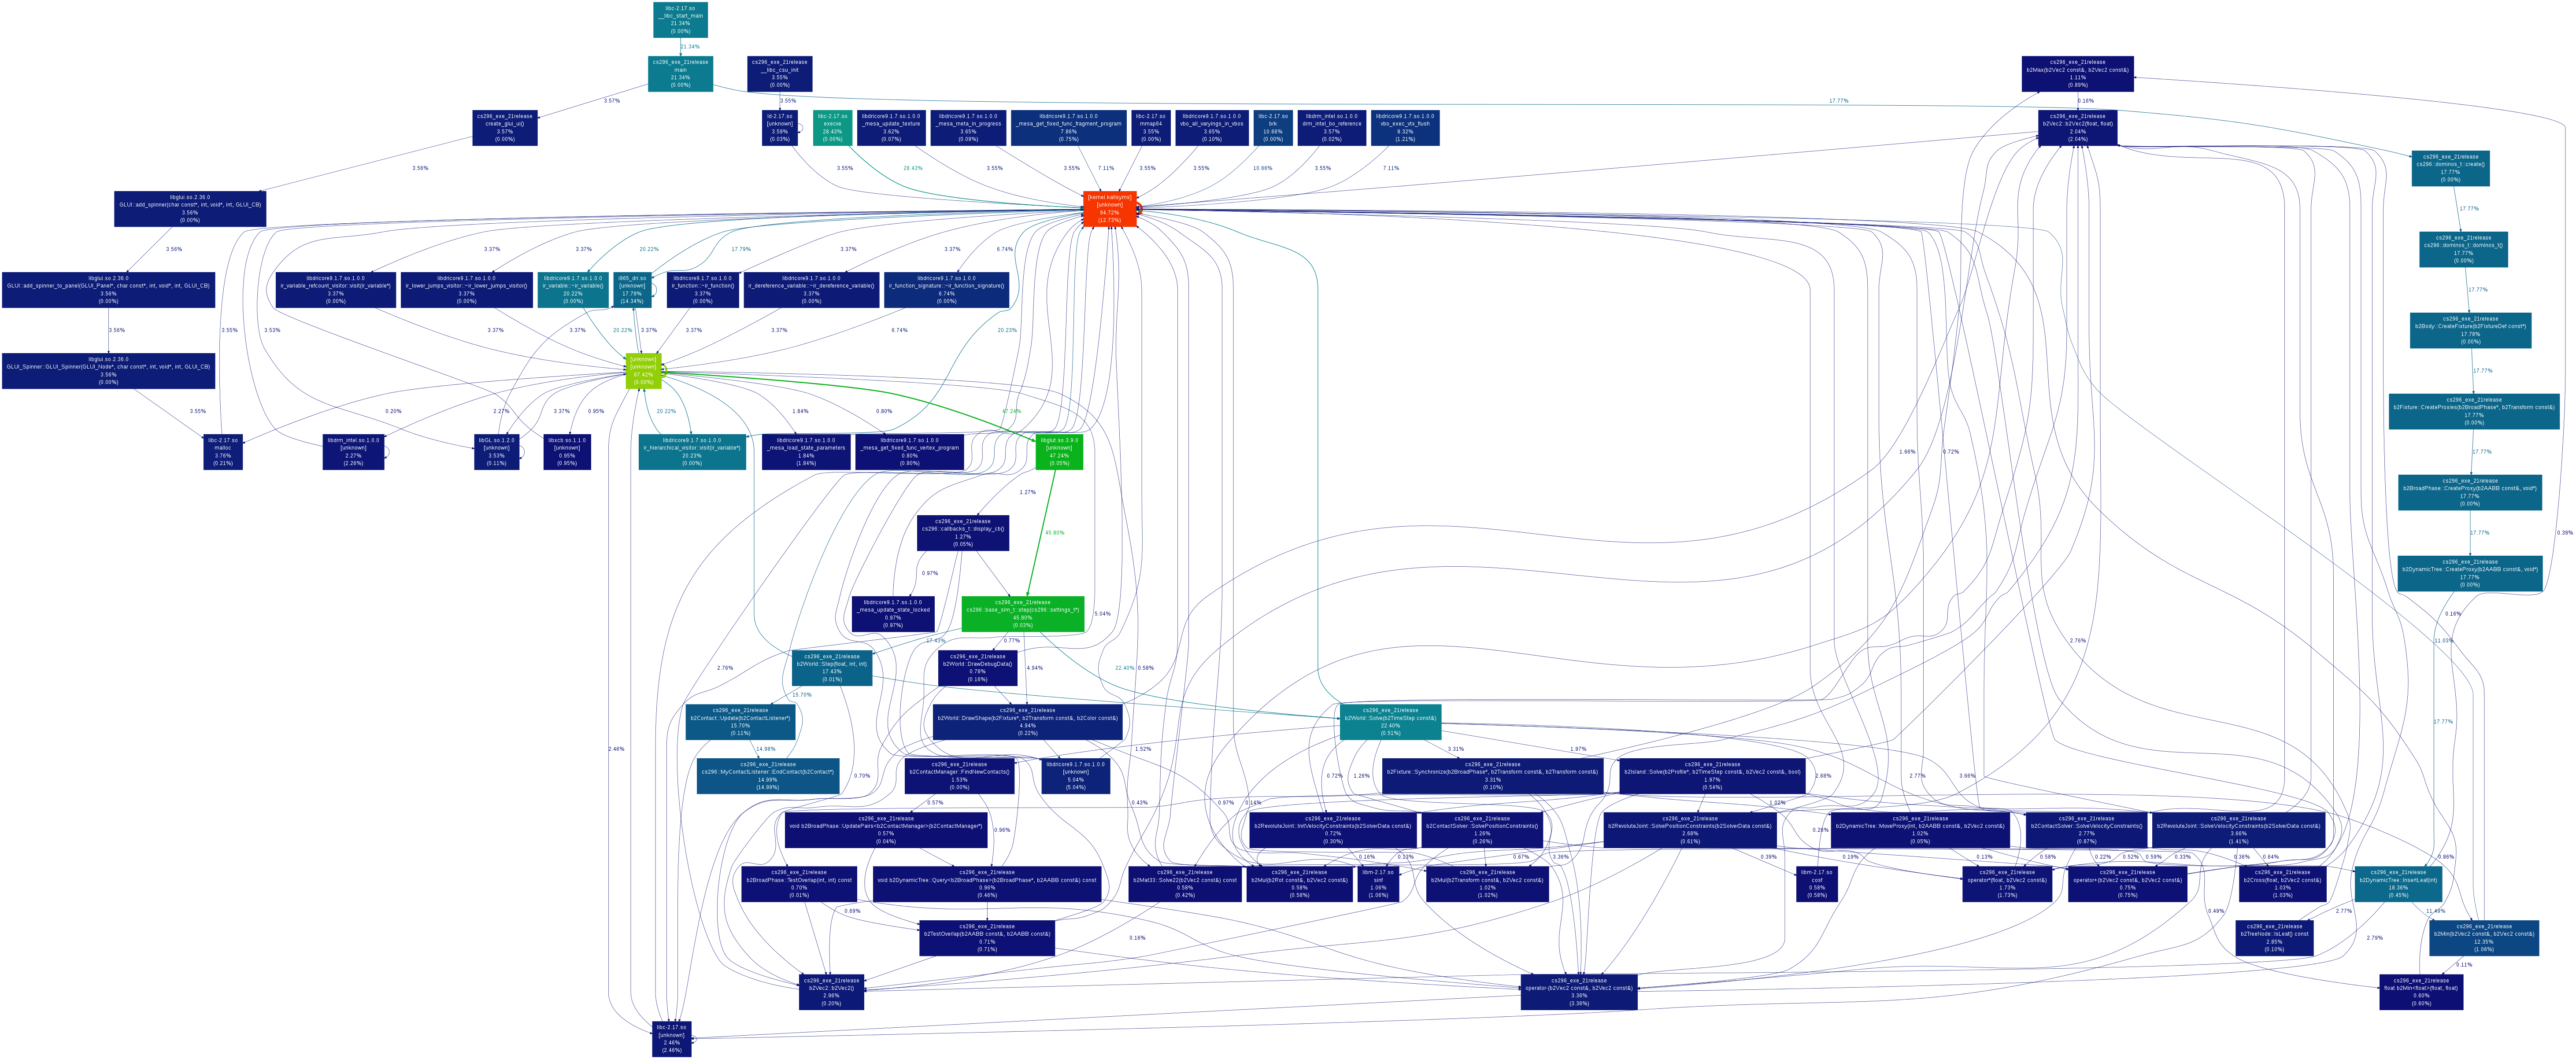
\includegraphics[scale=0.1]{../plots/releaseoutput.png}\\
Call Graph for Release
\end{center}
\begin{center}
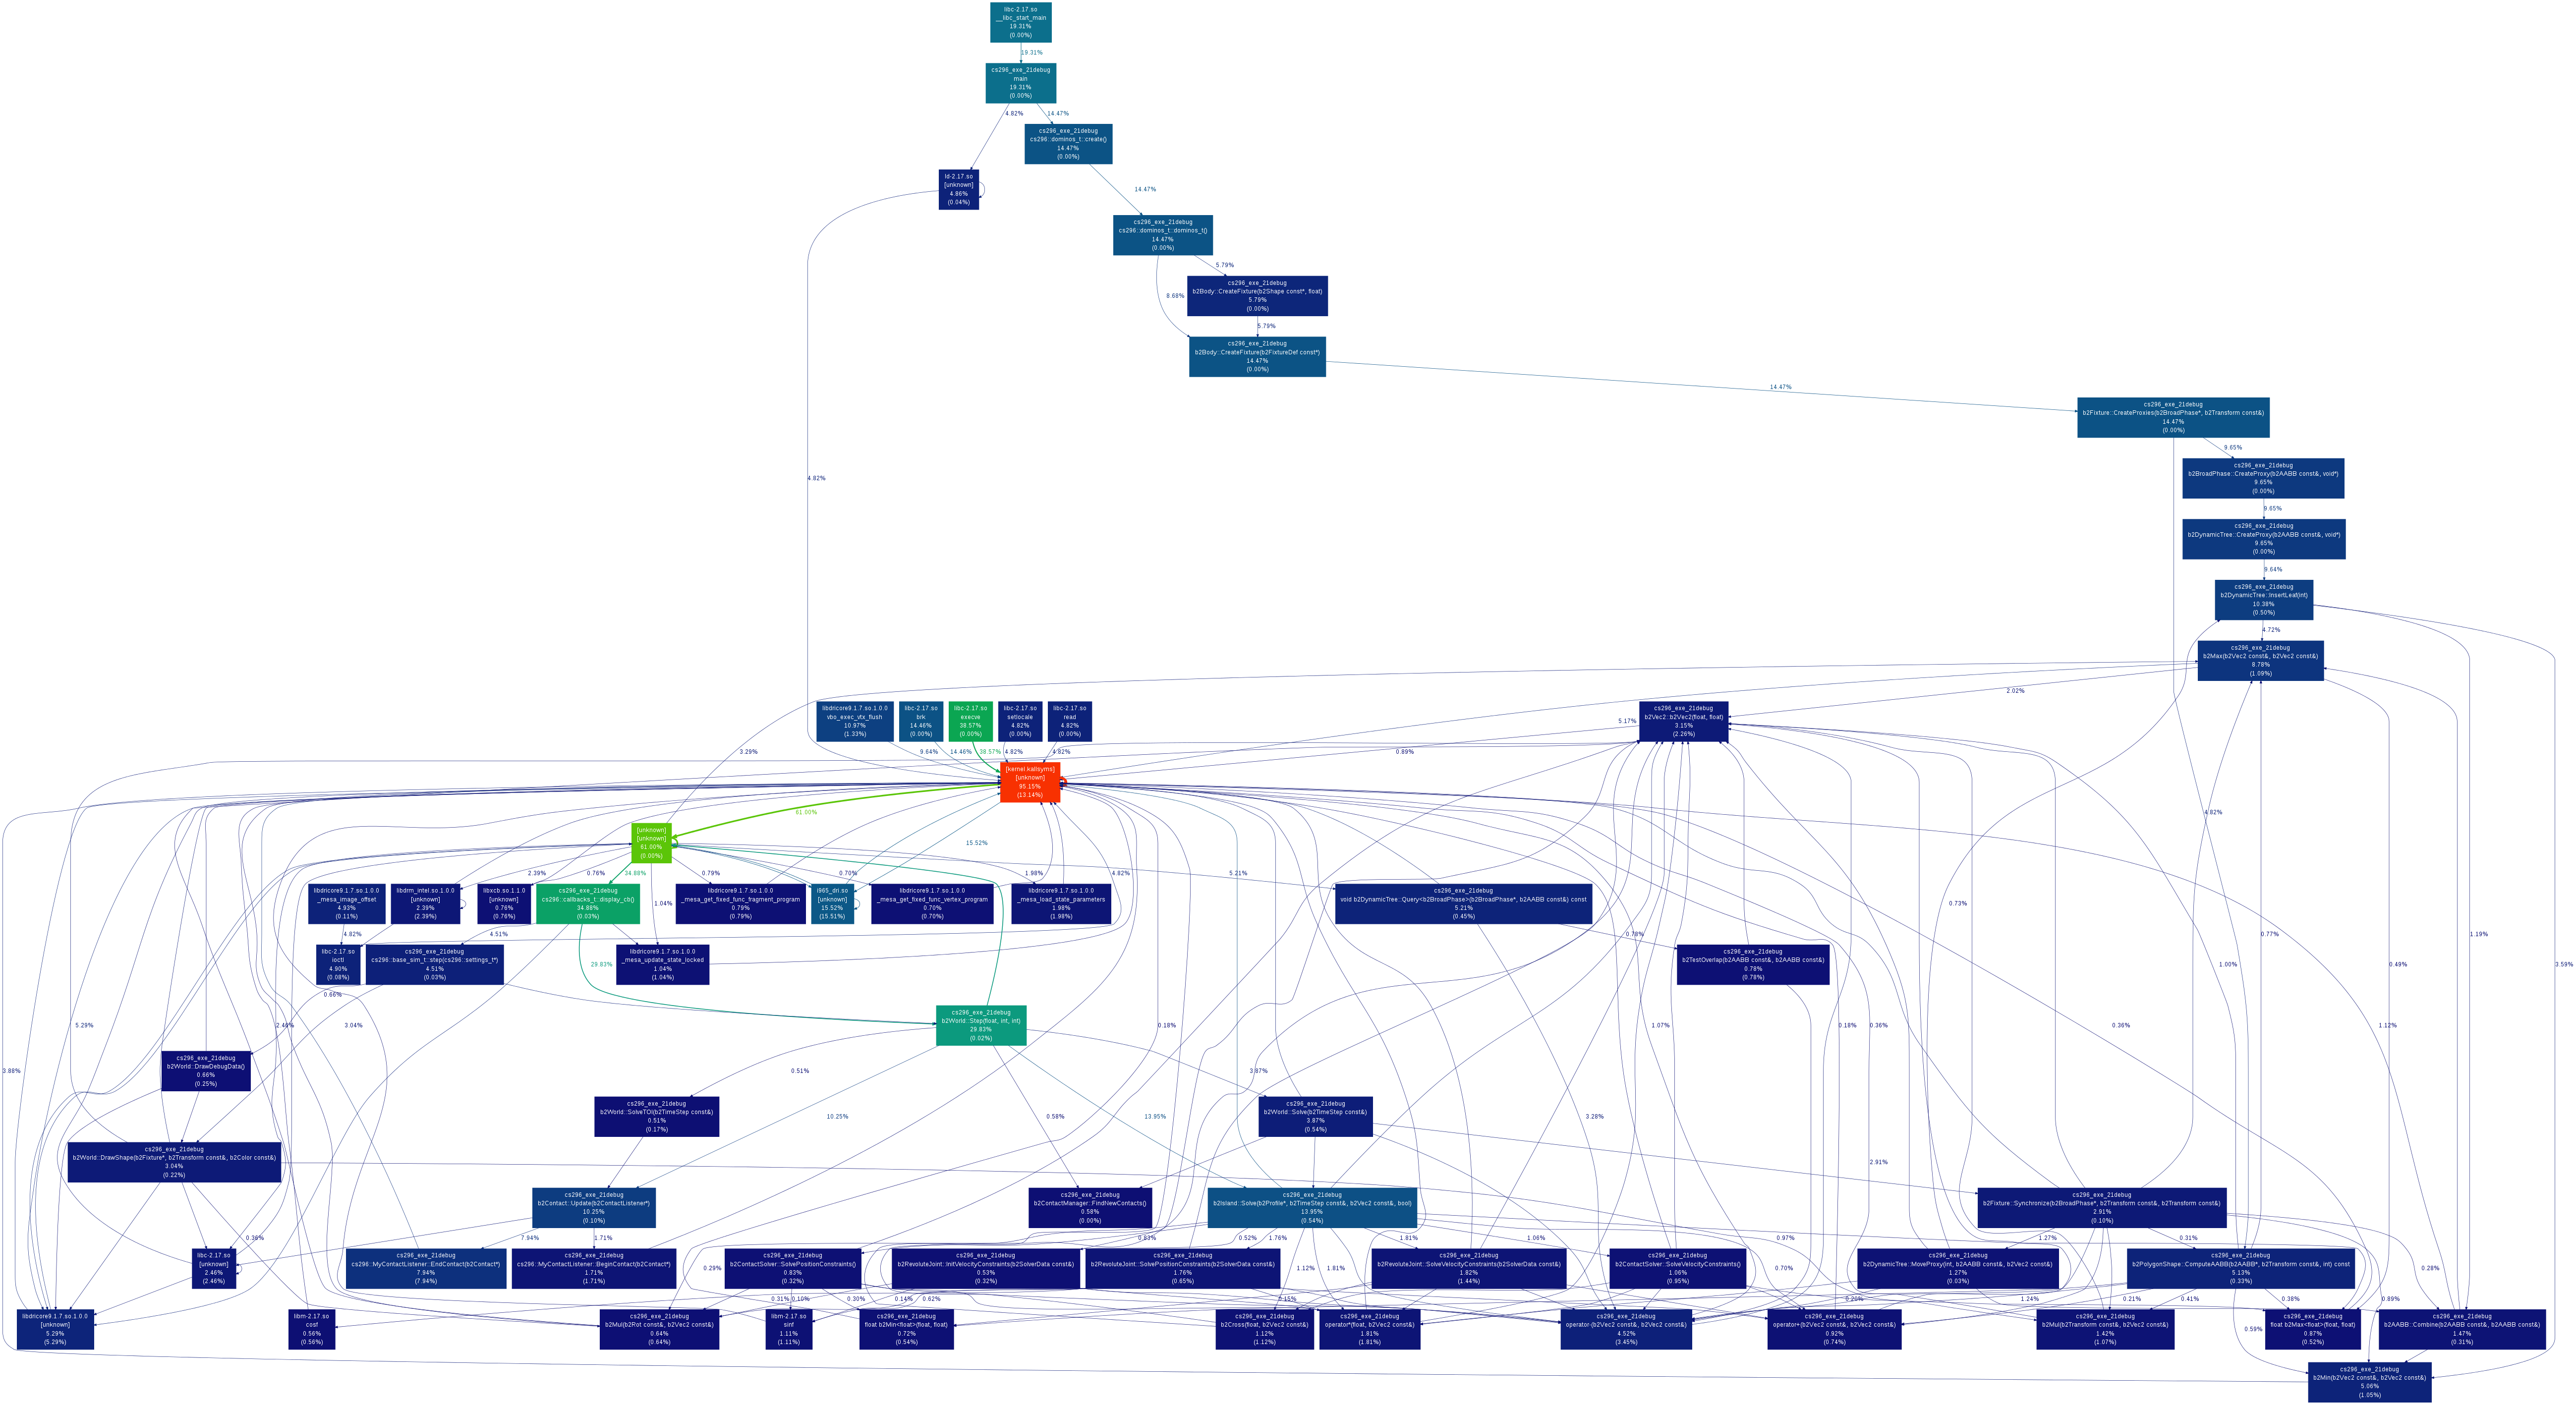
\includegraphics[scale=0.1]{../plots/debugoutput.png}\\
Call graph for Debug
\end{center}

\section{Timing Analysis from Lab 05}
\subsection{Interesting Things}
\subsubsection{Plot 1}
Average Loop Time increases as we increase the number of iterations because there is only one loop but the total time spent in that is continuously increasing with the increase in number of iterations.
Average Step time decreases exponentially as we increase the number of iterations (with an exception in the middle when it suddenly increases a little). This is because the initial steps take more time as compared to the later steps. The rate of change of average loop time is the step time at that value of iteration.\\
\begin{figure}
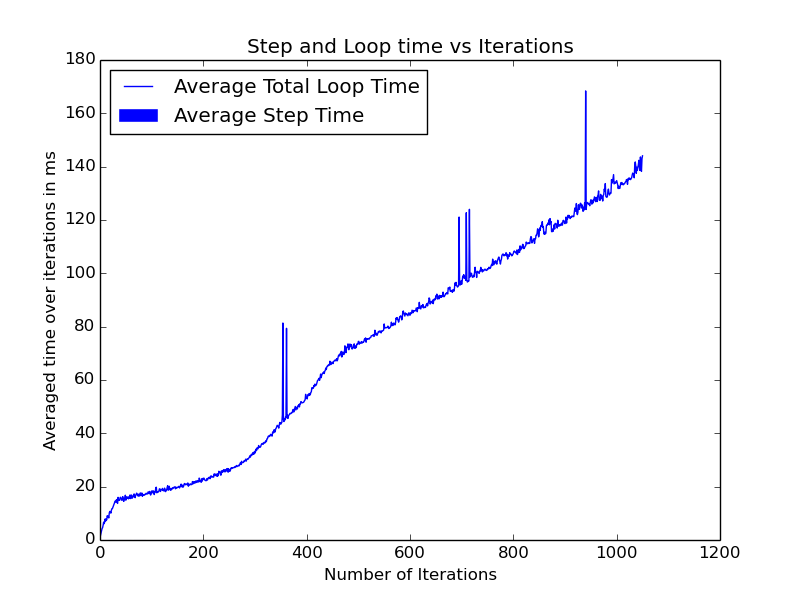
\includegraphics[scale=0.5]{../plots/g21_plot01.png}
\end{figure}
\subsubsection{Plot 2}
Average Step Time \textless Sum of velocity and position and collision time \textless  Velocity Time \textless  Position Time \textless Collision Time
The average position time and collision time are almost the same.\\
\begin{center}
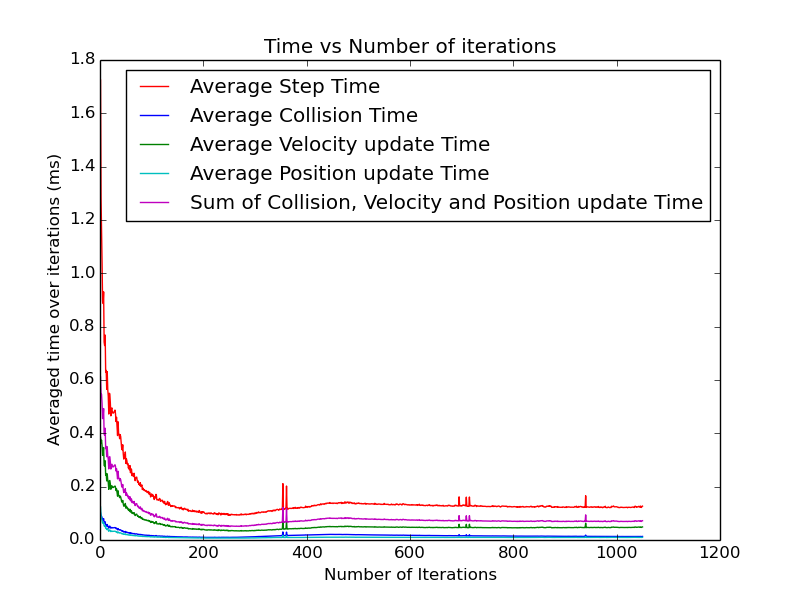
\includegraphics[scale=0.5]{../plots/g21_plot02.png}
\end{center}
\subsubsection{Plot 3}
Errors in average data time decreases as the number of iterations increase as errors get nullified with the increase in data points (iteration number) which appear in the denominator while taking the average.\\
\begin{center}
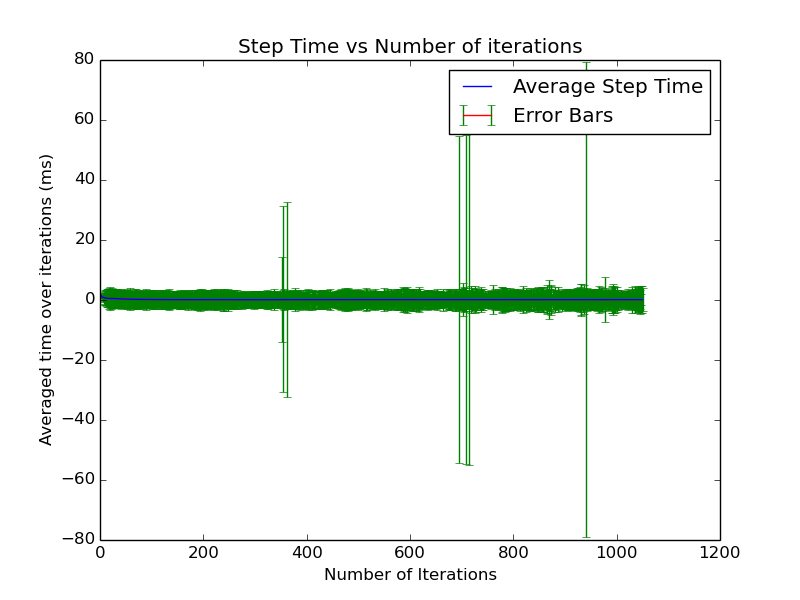
\includegraphics[scale=0.5]{../plots/g21_plot03.png}
\end{center}
\subsubsection{Plot 4}
Iterations with low step time are in high frequency while iterations with high step time are in low frequency. This is in accordance
with our plot for average step time vs iterations, as step time is quite low for all iteration values above a particular iteration, and
is high only for low iteration values.\\
\begin{center}
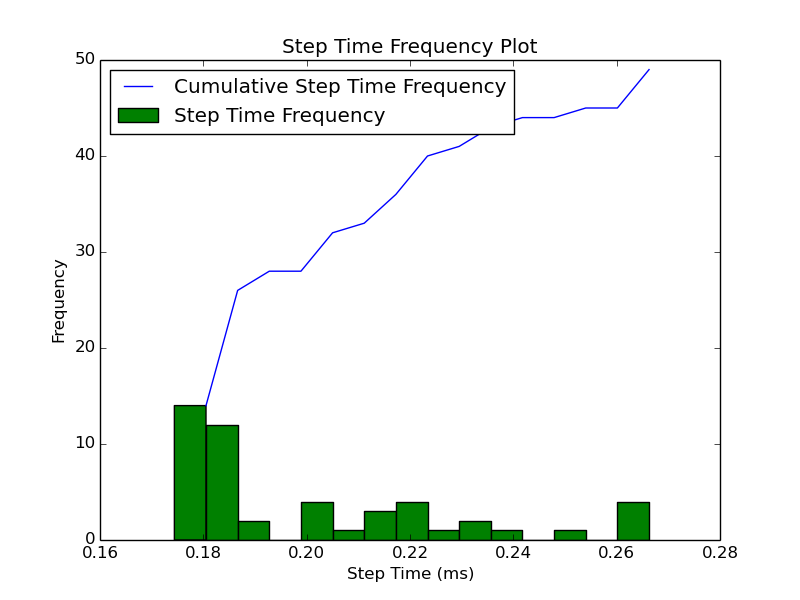
\includegraphics[scale=0.5]{../plots/g21_plot04.png}
\end{center}
\subsubsection{Plot 5}
Average step time for all reruns is very different from average step time for some random no of reruns for small iteration values
because the variation in step time is quite large. However, for high iteration values, average step time is almost the same for any no of
rerun values as variation in step time decreases.\\
\begin{center}
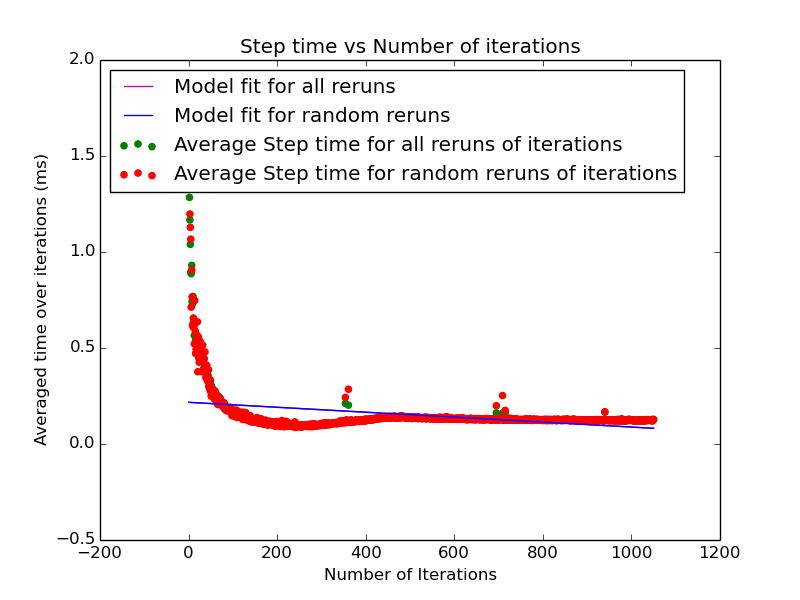
\includegraphics[scale=0.5]{../plots/g21_plot05.png}
\end{center}

\section{conclusion}
Now, we have explained all the new box2d elements added by us . Each element is simulated by some physics laws which are also mentioned.
We also reffered to links\cite{cs296_21:1} \cite{cs296_21:2} \cite{cs296_21:3} and books like \cite{book1}
\bibliographystyle{plain}
\bibliography{citations}
\end{document}
